\documentclass[conference]{IEEEtran}

\usepackage[spanish]{babel}
\usepackage[utf8]{inputenc} % Ensure the use of UTF-8 encoding
\usepackage{cite}
\usepackage{amsmath,amssymb,amsfonts}
\usepackage{algorithmic}
\usepackage{graphicx}
\usepackage{textcomp}
\usepackage{xcolor}

\def\BibTeX{{\rm B\kern-.05em{\sc i\kern-.025em b}\kern-.08em
    T\kern-.1667em\lower.7ex\hbox{E}\kern-.125emX}}

\begin{document}

\title{Boosting KMeans con KDTrees}

\author{\IEEEauthorblockN{Fernando Ramirez Arredondo\IEEEauthorrefmark{1}, Sixto Manuel Cáceres Terrones\IEEEauthorrefmark{2}}
\IEEEauthorblockA{\IEEEauthorrefmark{1}CS-UCSP, Email: fernando.ramirez@ucsp.edu.pe}
\IEEEauthorblockA{\IEEEauthorrefmark{2}CS-UCSP, Email: sixto.caceres@ucsp.edu.pe}
}

\maketitle

\begin{abstract}
    Este trabajo evalúa la eficiencia de integrar la estructura de datos KDTree en el algoritmo de clustering KMeans. Utilizando KDTree para la búsqueda de vecinos más cercanos, se logra una reducción significativa en el tiempo de ejecución, especialmente en conjuntos de datos grandes y con un número moderado a alto de clústeres. Los resultados experimentales demuestran que KMeans con KDTree ofrece una mejora sustancial en eficiencia computacional en comparación con la implementación estándar.
\end{abstract}

\begin{IEEEkeywords}
    KDTree, KMeans, Clustering, SIXTree
\end{IEEEkeywords}

\section{Introducción}
Una de las aplicaciones más conocidas dela búsqueda del vecino más cercano es en los algoritmos de clustering. El clustering es la forma principal de aprendizaje no supervisado. Los algoritmos de clustering toman un conjunto de datos sin etiquetar e intentan recopilar la mayor cantidad de información posible sobre su estructura, agrupando puntos de datos similares y separando los diferentes. El algoritmo más comun de clustering es KMeans. Una de las principales desventajas de KMeans es el cálculo fuerza bruta que realiza al calcular distancias entre los puntos y los centroides, KDTree puede ser utilizado para evitar calculos costosos y conseguir una mejor implementación\cite{samet1988overview}\cite{bentley1975multidimensional}. Las siguientes secciones describen tal implementación y sus resultados.

\section{Marco teórico}
\subsection{Algoritmo KMeans}
El algoritmo KMeans es un método de agrupamiento no supervisado ampliamente utilizado para dividir un conjunto de datos en $k$ grupos o clusters, donde $k$ es un parámetro predefinido. El proceso iterativo del algoritmo incluye los siguientes pasos.
\begin{itemize}
\item{Inicialización.} Selección aleatoria de $k$ puntos como centroides iniciales.
\item{Asignación de Clusters.} Asignación de cada punto de datos al cluster cuyo centroide está más cercano.
\item{Actualización de Centroides.} Recalcular los centroides como la media de los puntos asignados a cada cluster.
\item{Repetición.} Repetir los pasos de asignación y actualización hasta que los centroides no cambien significativamente o se alcance un número máximo de iteraciones.
\end{itemize}

\subsection{Complejidad Computacional de KMeans}
La complejidad del algoritmo KMeans es aproximadamente  $O(t \cdot n \cdot k \cdot d)$, donde $t$ es el número de iteraciones, $n$ es el número de puntos de datos, $k$ es el número de clusters y $d$ es la dimensionalidad de los datos. El cálculo de distancias en cada iteración representa la mayor parte del costo computacional.

\subsection{Estructura de Datos KDTree}
El KDTree (K-dimensional tree) es una estructura de datos que facilita la búsqueda eficiente de vecinos más cercanos en un espacio multidimensional. Se utiliza para particionar el espacio de datos en regiones y permite realizar consultas de proximidad de manera eficiente.
\begin{itemize}
    \item{Construcción.} La construcción de un KDTree tiene una complejidad de $O(n \cdot log n)$.
    \item{Búsqueda de Vecinos Más Cercanos.} La búsqueda de vecinos más cercanos tiene una complejidad promedio de $O(log n)$ en espacios de baja dimensionalidad.
\end{itemize}
\subsection{Integración de KDTree con KMmeans}
El uso de KDTree en el algoritmo KMeans se centra en la fase de asignación de clusters. En lugar de calcular la distancia de cada punto de datos a todos los centroides, se utiliza el KDTree para encontrar el centroide más cercano de manera más eficiente, reduciendo así el número de cálculos de distancia necesarios.
\begin{itemize}
    \item{Beneficios.} Reducción del tiempo de ejecución, especialmente en conjuntos de datos grandes.
    \item{Limitaciones.} La eficiencia de KDTree disminuye en espacios de alta dimensionalidad, y la necesidad de reconstruir el KDTree en cada iteración añade una sobrecarga computacional.
\end{itemize}
\subsection{Evaluación de Desempeño}
La evaluación del rendimiento del algoritmo KMeans con y sin KDTree incluye.
\begin{itemize}
\item{Medición del Tiempo de Ejecución.} Comparación directa de los tiempos de ejecución para diferentes configuraciones de parámetros.
\end{itemize}

\section{Metodología}
El objetivo del estudio es evaluar la eficiencia y eficacia de la integración de la estructura de datos KDTree en el algoritmo KMeans, comparando su rendimiento con el KMeans estándar en términos de tiempo de ejecución y precisión en la asignación de clusters.

\subsection{Diseño del Experimento}
\subsubsection{Selección de Datos}
Utilizar conjuntos de 2400 datos sintéticos con diferentes tamaños de en formato punto flotante y dimensionalidad 2.
\subsubsection{Implementación de Algoritmos}
Implementar el algoritmo KMeans estándar (código fuente en repositorio). 
El algoritmo KMeans estándar tiene dos fases principales en cada iteración.
\begin{itemize}
\item{Asignación de Clusters.} Calcular la distancia de cada punto de datos a cada centroide y asignar el punto al cluster más cercano. \(O(n \cdot k \cdot d)\).
\item{Actualización de Centroides.} Recalcular los centroides como la media de todos los puntos asignados a cada cluster. \(O(n \cdot d)\) (generalmente menor en comparación con la asignación de clusters).
\end{itemize}
Para \(n\) puntos de datos, \(k\) clusters, \(d\) dimensiones, y \(t\) iteraciones.
En general, la complejidad total del KMeans estándar es \(O(t \cdot n \cdot k \cdot d)\).
Implementar el algoritmo KMeans mejorado con KDTree(código fuente en repositorio).
El uso de KDTree se centra en optimizar la fase de asignación de clusters. La complejidad se divide en.
\begin{itemize}
    \item{Construcción del KDTree.} Se realiza con los centroides en cada iteración. La complejidad es \(O(k \cdot \log k)\) para construir el KDTree con \(k\) centroides.
    \item{Búsqueda de Vecinos Más Cercanos.} Usar KDTree para encontrar el centroide más cercano a cada punto de datos. La complejidad promedio es \(O(\log k)\) por búsqueda.
\end{itemize}
Para \(n\) puntos de datos, \(k\) clusters, \(d\) dimensiones, y \(t\) iteraciones.
\begin{itemize}
    \item{Construcción del KDTree.} \(O(t \cdot k \cdot \log k)\)
    \item{Asignación de Clusters con KDTree.} \(O(t \cdot n \cdot \log k \cdot d)\)
\end{itemize}

En general, la complejidad total del KMeans con KDTree es \(O(t \cdot (n \cdot \log k \cdot d + k \cdot \log k))\).
\subsubsection{Parámetros del Experimento}
Variar el número de clusters k (por ejemplo, 5, 15, 25, 50, 75).
Variar la cantidad de datos n (por ejemplo, 1000, 1150, 1300, 1450, 1600, 1750, 1900, 2050, 2200, 2400).
Fijar un número máximo de iteraciones para asegurar la convergencia, consideramos 12 como el número pertinente.
\subsection{Evaluación del Rendimiento}
\subsubsection{Tiempo de Ejecución}
Medir el tiempo de ejecución de ambos algoritmos en cada configuración de parámetros.
\subsection{Análisis de Resultados}
Comparar los tiempos de ejecución para diferentes configuraciones de datos y clusters.
Utilizar herramientas de visualización para presentar los resultados de manera clara (gráficos de líneas, tablas comparativas).

\section{Resultados y Discusión}
Los experimentos que hacen uso del KDTree para reducir el costo computacional de la implementación demuestran bajo aumento de tiempo conforme aumentan los parametros. Observando Fig. \ref{fig:kmeanskdtree}, el aumento en el número de clusters no tiene mucho efecto en el desempeño, por el contrario, un número muy pequeño de clusters como 5 o 15 tiene efectos negativos. Observando Fig. \ref{fig:kmeanskdtree_six}, el aumento en el número de datos tampoco parece tener efectos negativos muy grandes, el desempeño se mantiene proporcional.
\newline
Los experimentos que hacen uso de fuerza bruta (KMeans sin KDtree), por otro lado, demuestran poca tolerancia al aumento de dimensionalidades. Observando Fig. \ref{fig:kmeans}, el aumento en el número de clusters es muy perjudicial para el desempeño del algoritmo de clustering, podemos observar una relación muy notoria entre el número de clusters y el desempeño para todas las cantidades de puntos. Observando Fig. \ref{fig:kmeans_six}, el aumento en el número de datos también tiende a empeorar el desempeño de programa, sin embargo, no es algo tan notorio. Teniendo en cuenta que el calculo fuerza bruta se realiza con cada cluster, es entendible que el desempeño no cambie mucho con una variacion de clusters pequeña.
\newline
Observando Fig. \ref{fig:kdtree1}-\ref{fig:kdtree10} existe variación en la definición de los clusters para los 2400 puntos utilizando KMeans. Observando Fig. \ref{fig:kmeans1}-\ref{fig:kmeans10}, encontramos resultados similares haciendo uso de KMeans+KDTree. Esto nos dice que KMeans no es deterministico, y mejorar la implementación haciendo uso de KDTree no tiene efecto en este sentido.
\begin{figure}[htbp]
    \centering
    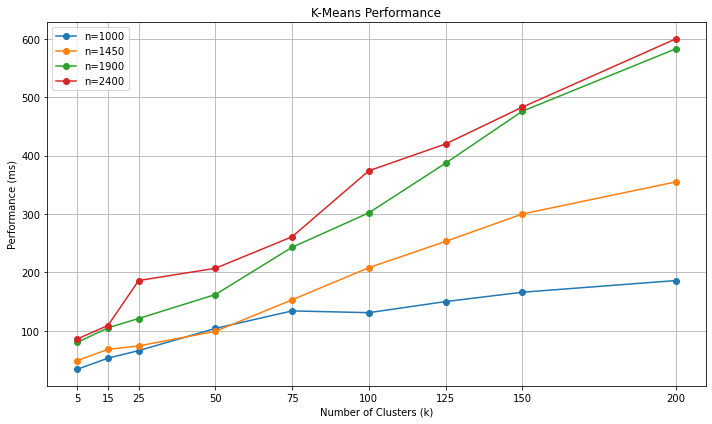
\includegraphics[width=1\linewidth]{figures/kmeans.png} % Adjust width as needed
    \caption{Ejecución de KMeans variando el número de clusters}
    \label{fig:kmeans}
\end{figure}

\begin{figure}[htbp]
    \centering
    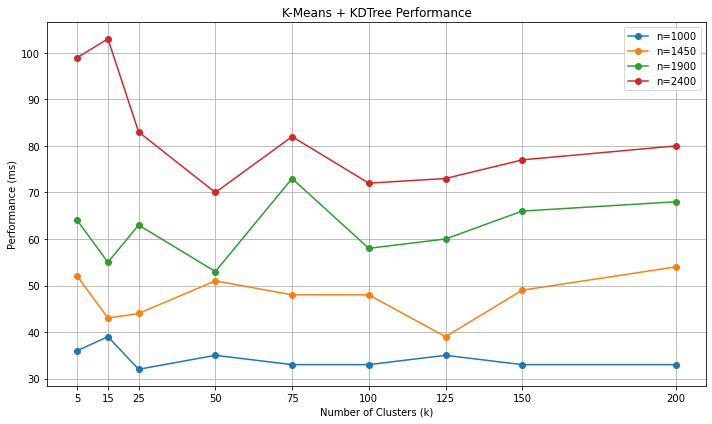
\includegraphics[width=1\linewidth]{figures/kmeanskdtree.png} % Adjust width as needed
    \caption{Ejecución de KMeans+KDTree variando el número de clusters}
    \label{fig:kmeanskdtree}
\end{figure}

\begin{figure}[htbp]
    \centering
    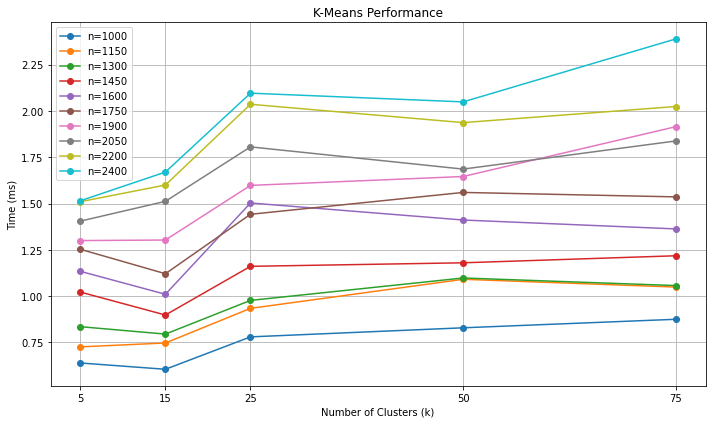
\includegraphics[width=1\linewidth]{figures/kmeans_six.png} % Adjust width as needed
    \caption{Ejecución de KMeans variando el número de datos}
    \label{fig:kmeans_six}
\end{figure}

\begin{figure}[htbp]
    \centering
    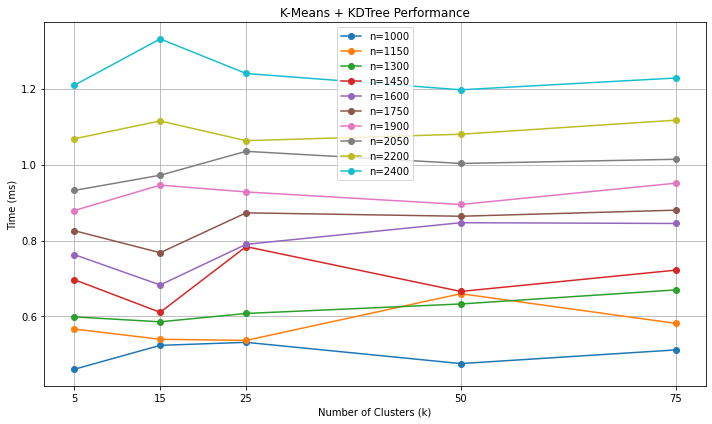
\includegraphics[width=1\linewidth]{figures/kmeanskdtree_six.png} % Adjust width as needed
    \caption{Ejecución de KMeans+KDTree variando el número de datos}
    \label{fig:kmeanskdtree_six}
\end{figure}
\begin{figure}[htbp]
    \centering
    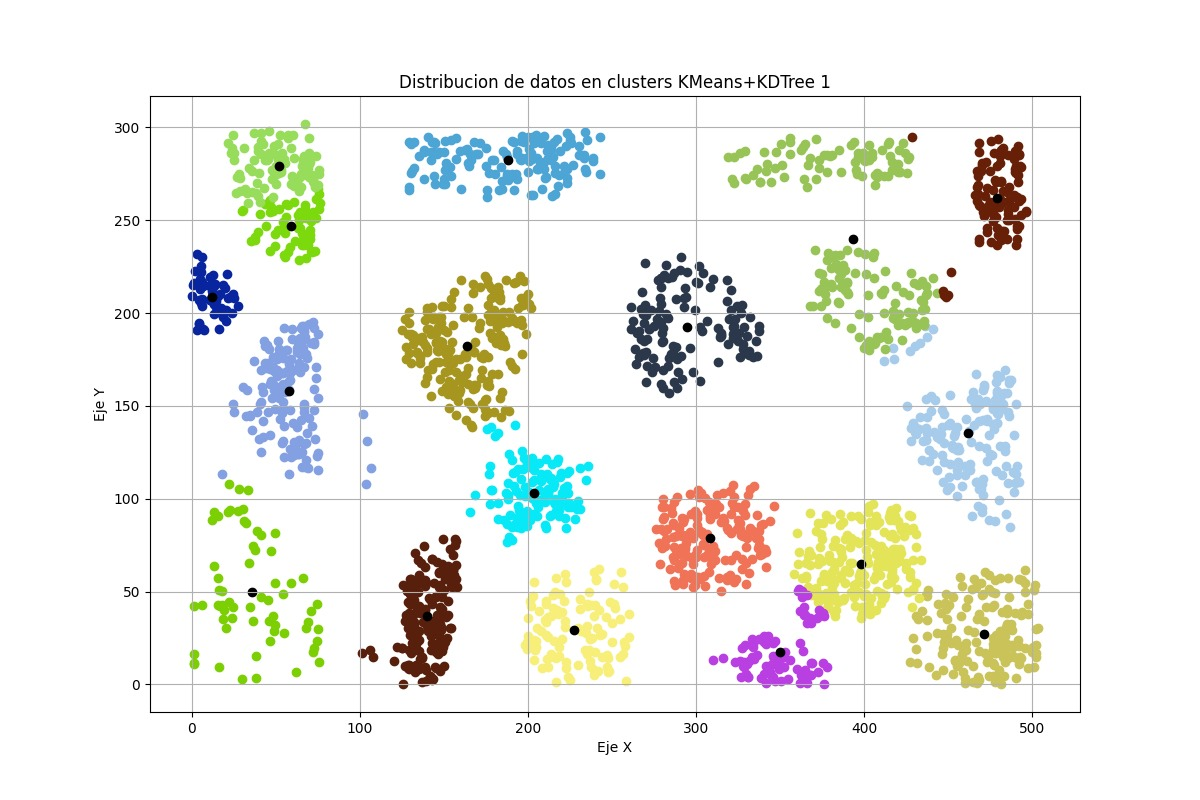
\includegraphics[width=1\linewidth]{figures/kdtree1.jpeg} % Adjust width as needed
    \caption{Distribucion de datos usando KMeans+KDTree}
    \label{fig:kdtree1}
\end{figure}
\begin{figure}[htbp]
    \centering
    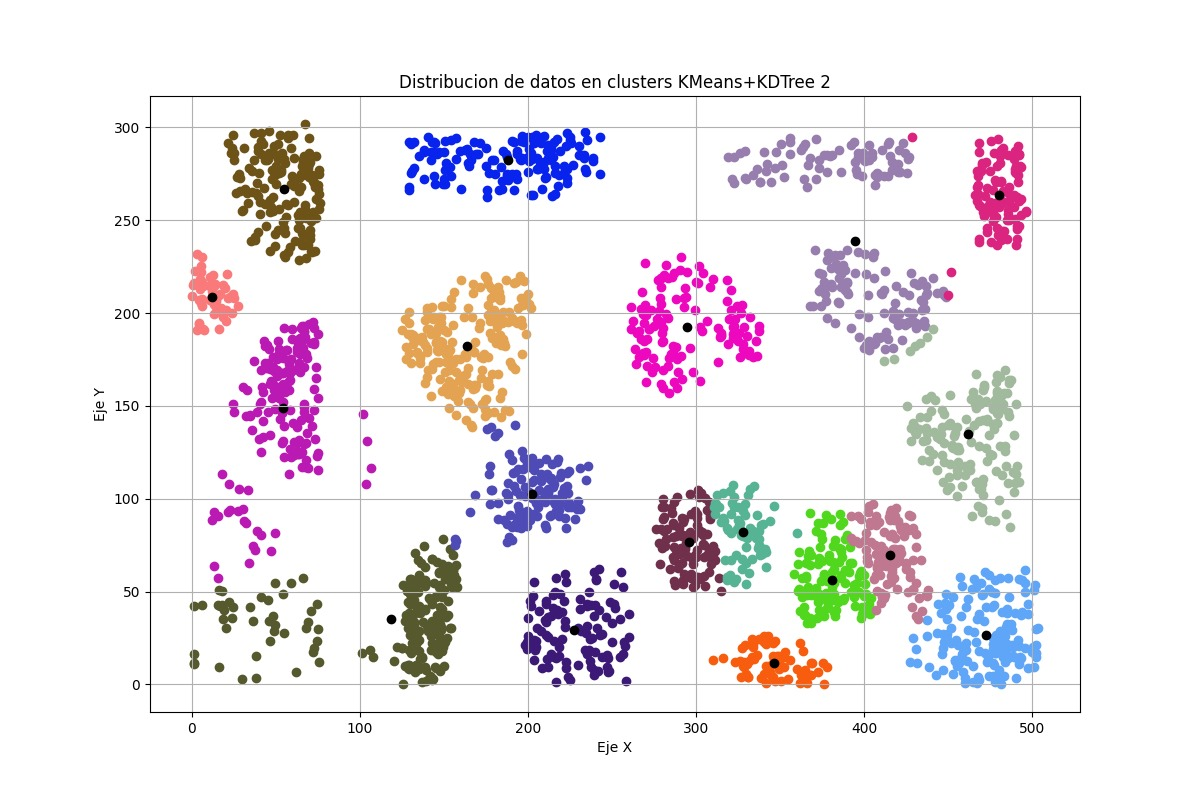
\includegraphics[width=1\linewidth]{figures/kdtree2.jpeg} % Adjust width as needed
    \caption{Distribucion de datos usando KMeans+KDTree}
    \label{fig:kdtree2}
\end{figure}
\begin{figure}[htbp]
    \centering
    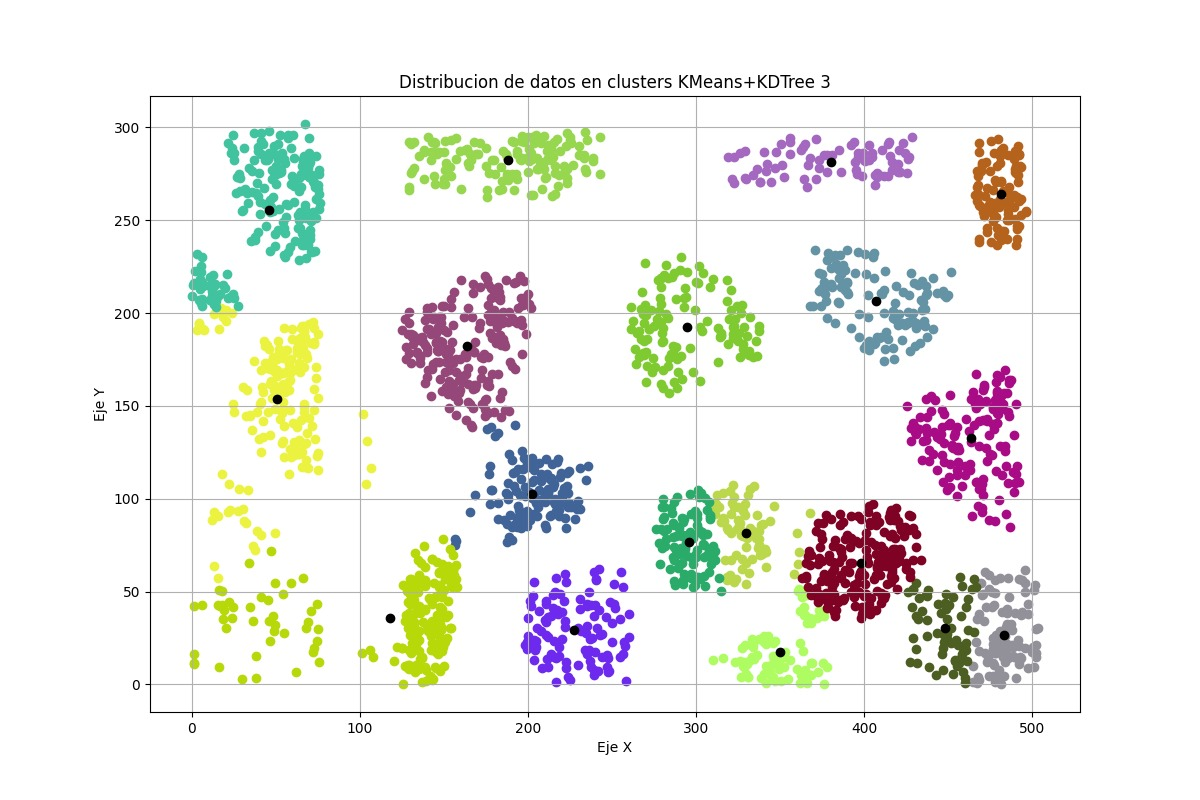
\includegraphics[width=1\linewidth]{figures/kdtree3.jpeg} % Adjust width as needed
    \caption{Distribucion de datos usando KMeans+KDTree}
    \label{fig:kdtree3}
\end{figure}
\begin{figure}[htbp]
    \centering
    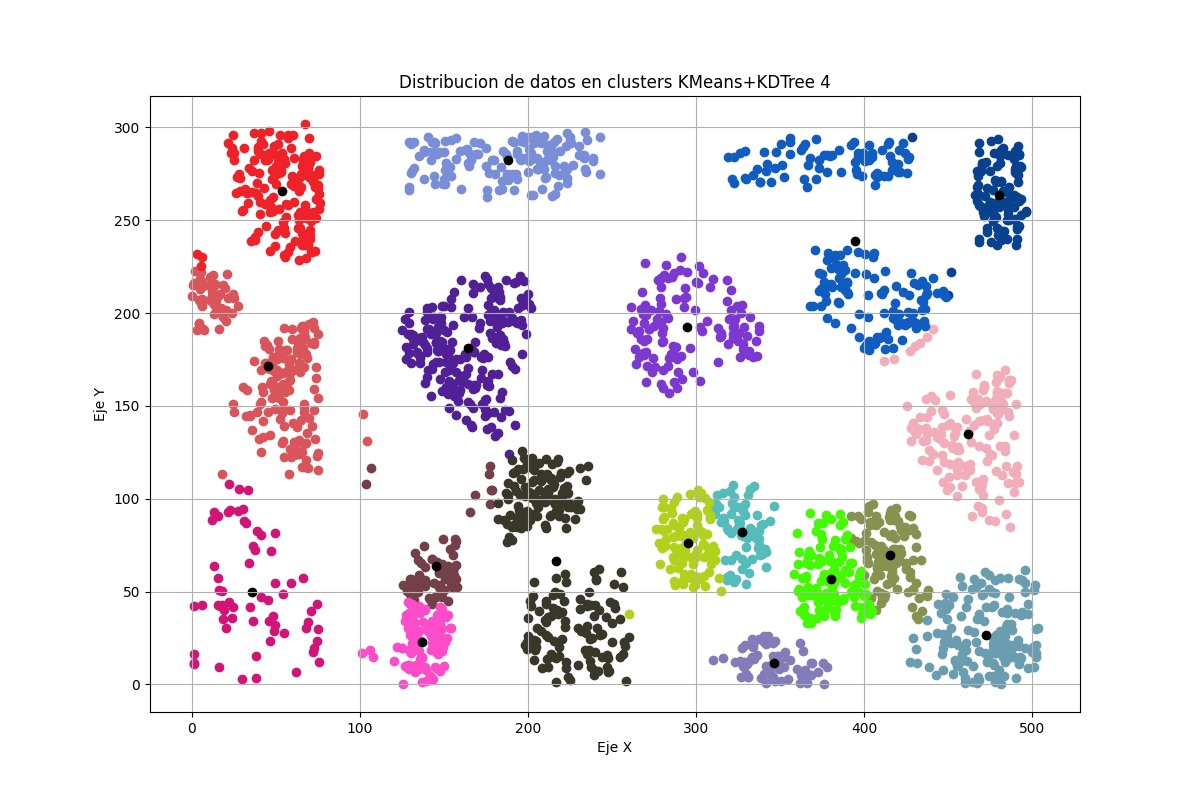
\includegraphics[width=1\linewidth]{figures/kdtree4.jpeg} % Adjust width as needed
    \caption{Distribucion de datos usando KMeans+KDTree}
    \label{fig:kdtree4}
\end{figure}
\begin{figure}[htbp]
    \centering
    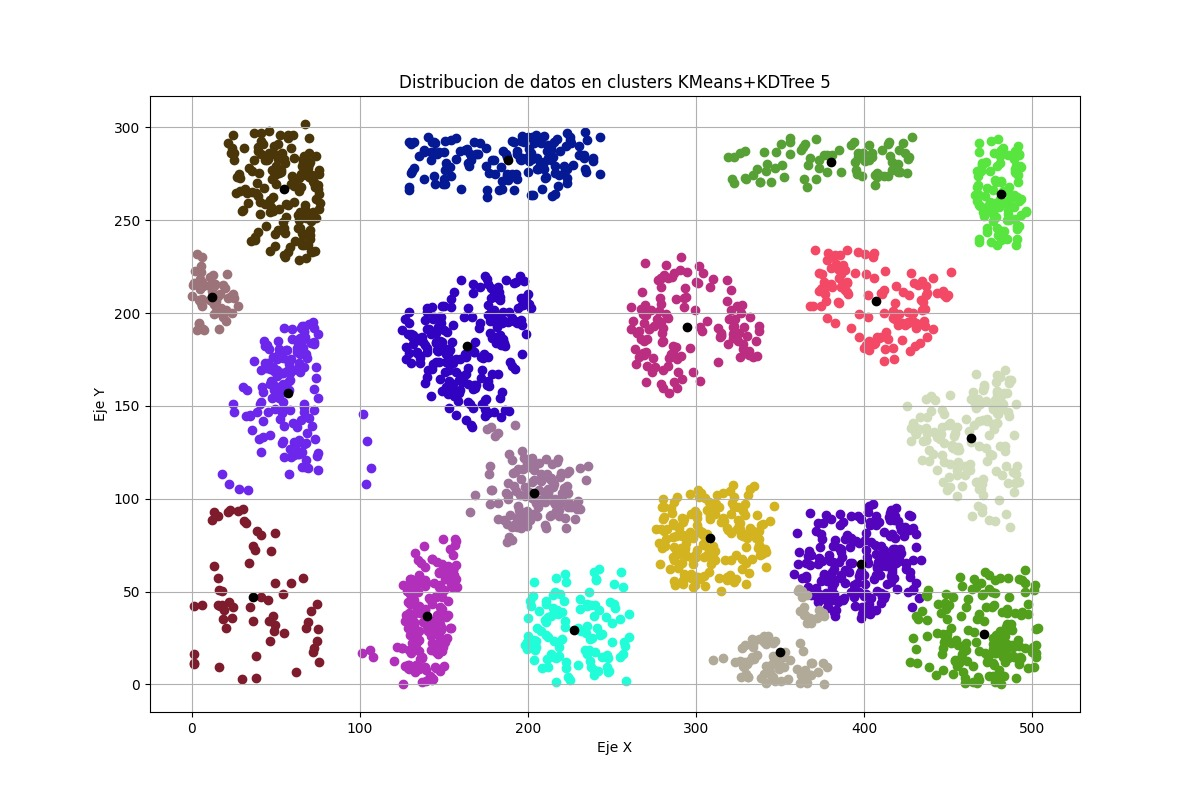
\includegraphics[width=1\linewidth]{figures/kdtree5.jpeg} % Adjust width as needed
    \caption{Distribucion de datos usando KMeans+KDTree}
    \label{fig:kdtree5}
\end{figure}
\begin{figure}[htbp]
    \centering
    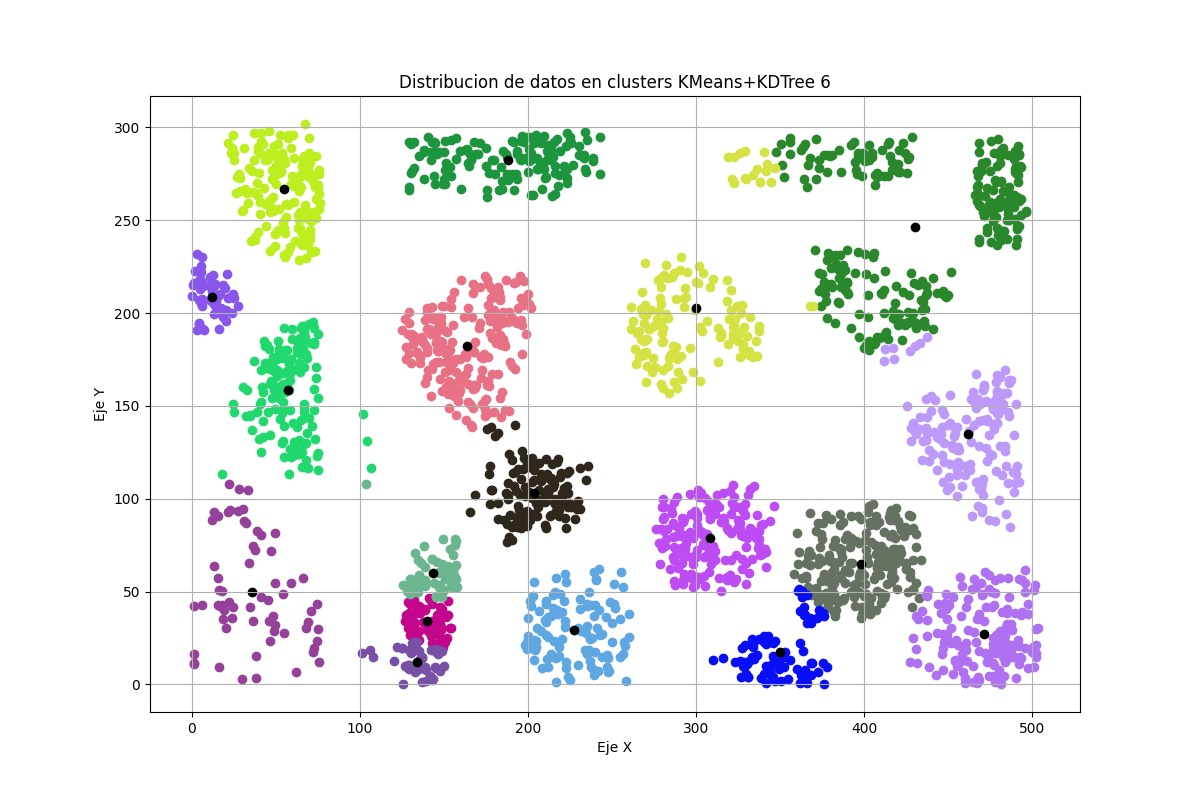
\includegraphics[width=1\linewidth]{figures/kdtree6.jpeg} % Adjust width as needed
    \caption{Distribucion de datos usando KMeans+KDTree}
    \label{fig:kdtree6}
\end{figure}
\begin{figure}[htbp]
    \centering
    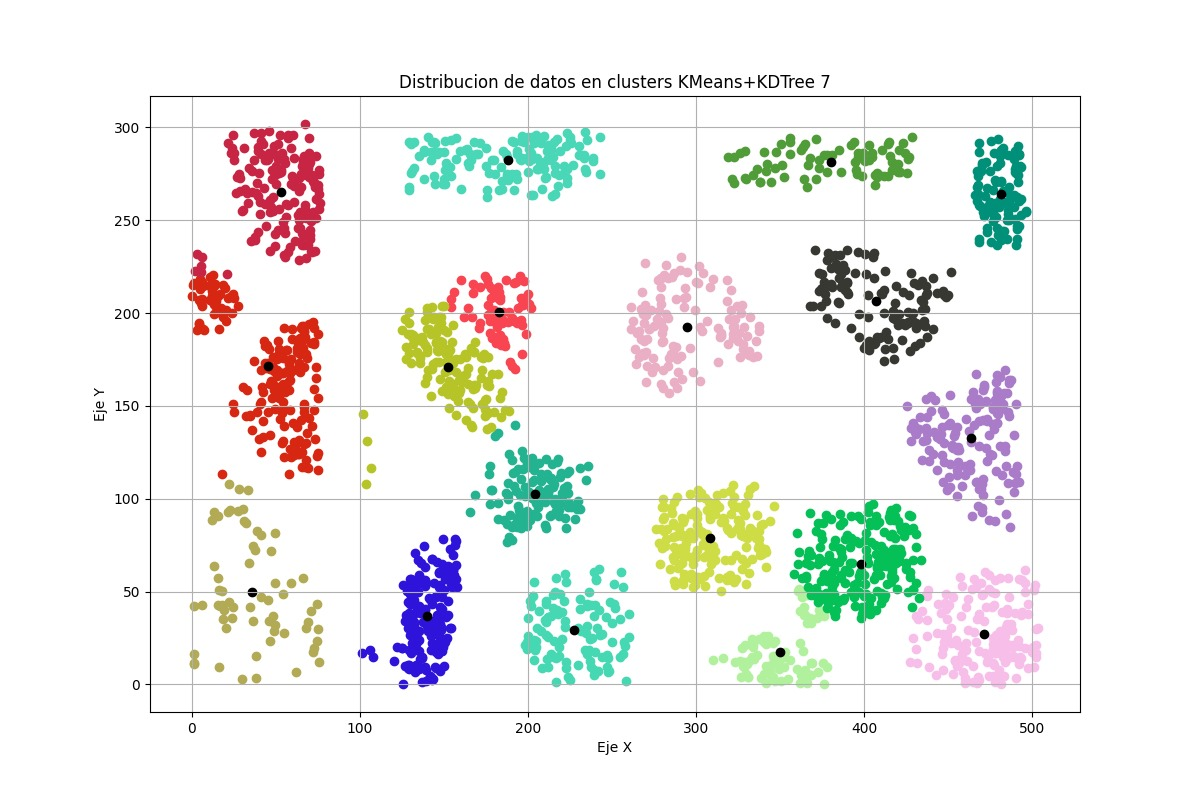
\includegraphics[width=1\linewidth]{figures/kdtree7.jpeg} % Adjust width as needed
    \caption{Distribucion de datos usando KMeans+KDTree}
    \label{fig:kdtree7}
\end{figure}
\begin{figure}[htbp]
    \centering
    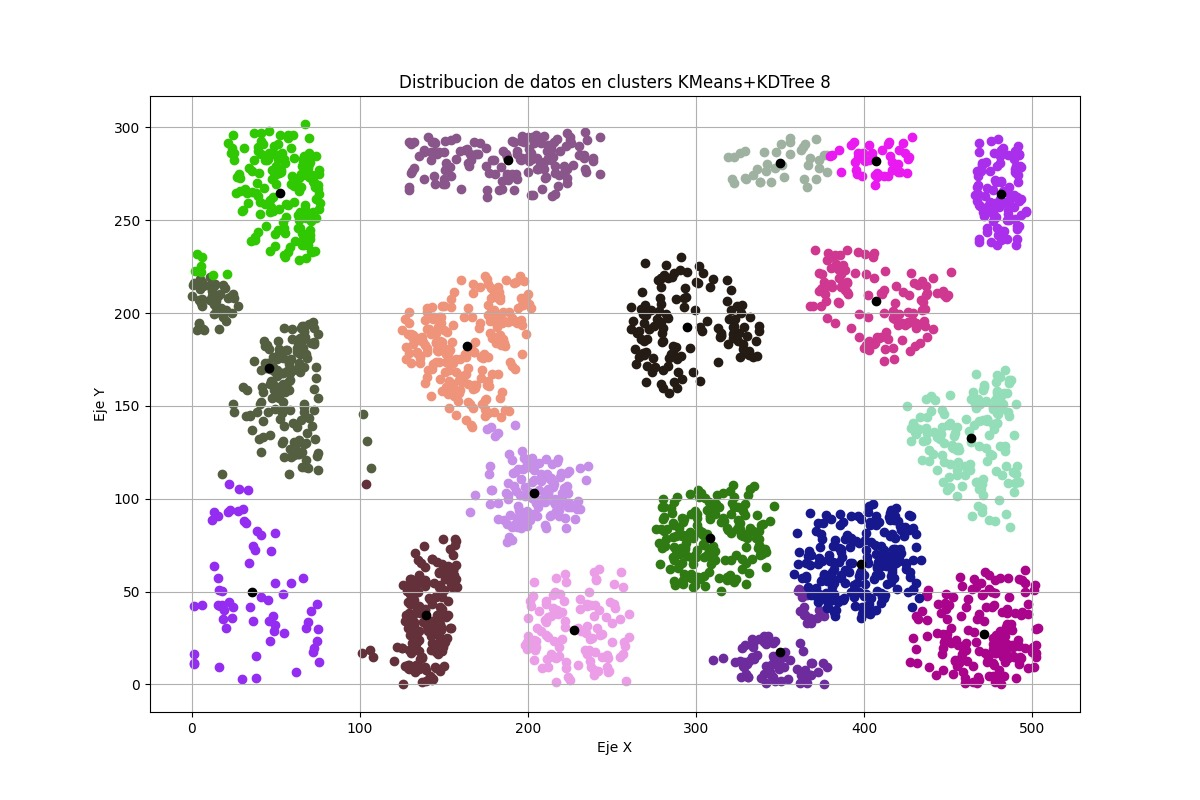
\includegraphics[width=1\linewidth]{figures/kdtree8.jpeg} % Adjust width as needed
    \caption{Distribucion de datos usando KMeans+KDTree}
    \label{fig:kdtree8}
\end{figure}
\begin{figure}[htbp]
    \centering
    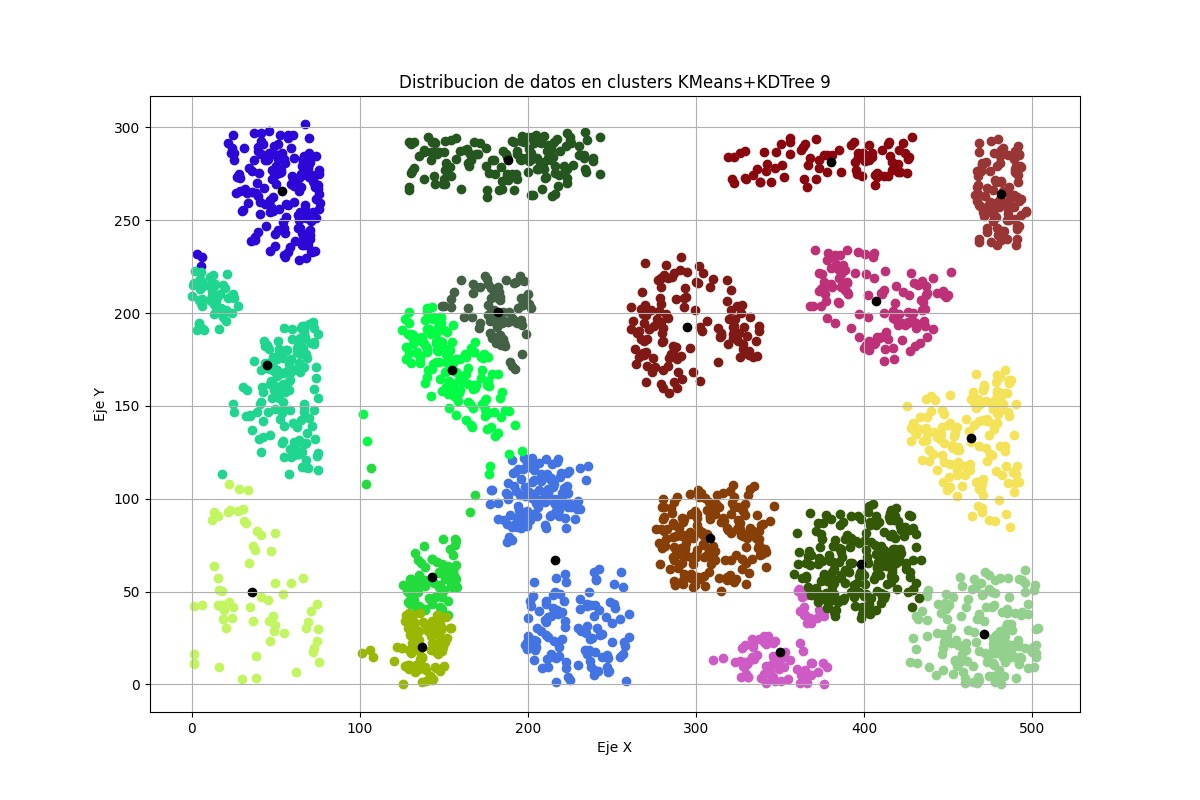
\includegraphics[width=1\linewidth]{figures/kdtree9.jpeg} % Adjust width as needed
    \caption{Distribucion de datos usando KMeans+KDTree}
    \label{fig:kdtree9}
\end{figure}
\begin{figure}[htbp]
    \centering
    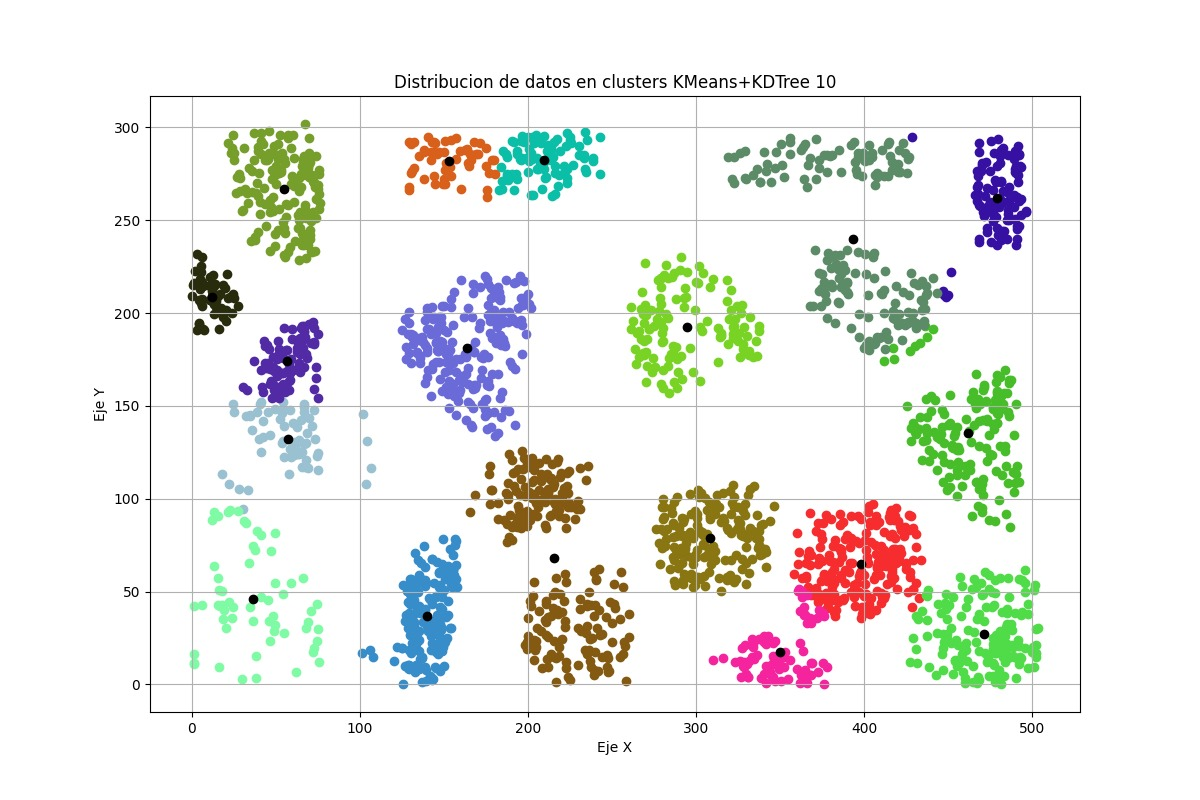
\includegraphics[width=1\linewidth]{figures/kdtree10.jpeg} % Adjust width as needed
    \caption{Distribucion de datos usando KMeans+KDTree}
    \label{fig:kdtree10}
\end{figure}

\begin{figure}[htbp]
    \centering
    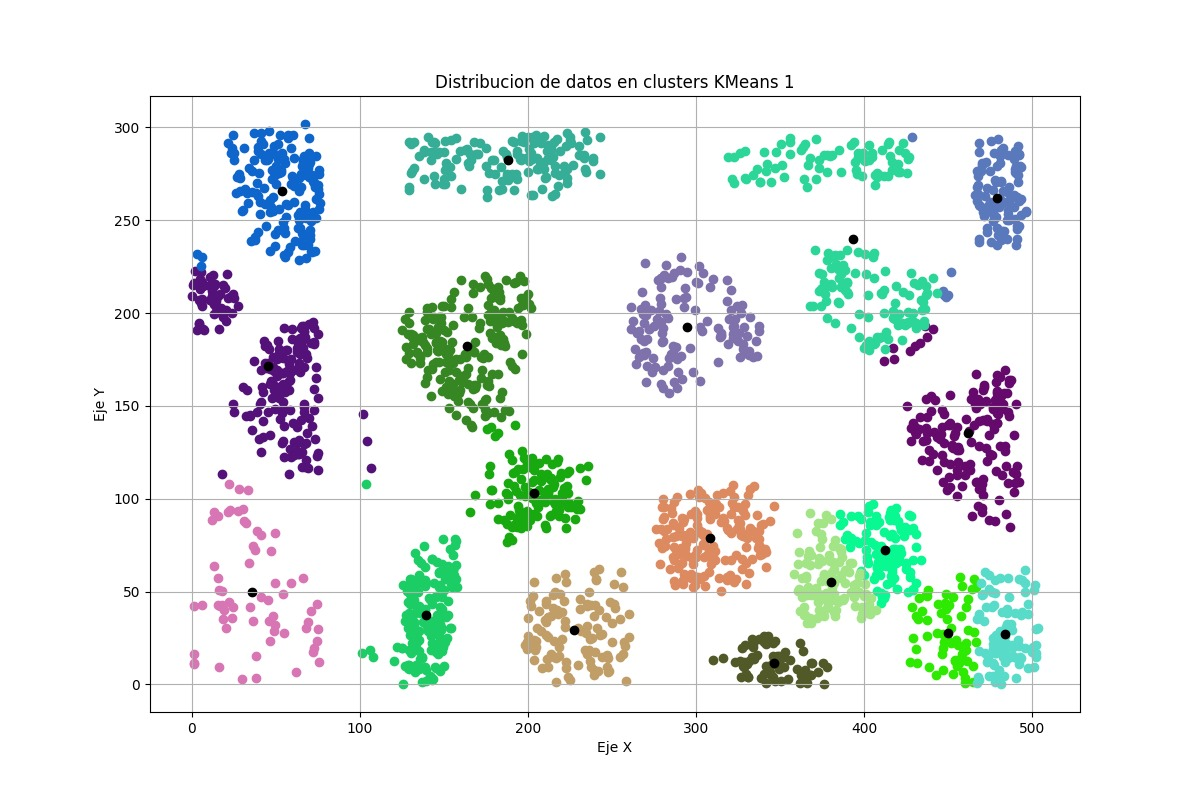
\includegraphics[width=1\linewidth]{figures/kmeans1.jpeg} % Adjust width as needed
    \caption{Distribucion de datos usando KMeans}
    \label{fig:kmeans1}
\end{figure}
\begin{figure}[htbp]
    \centering
    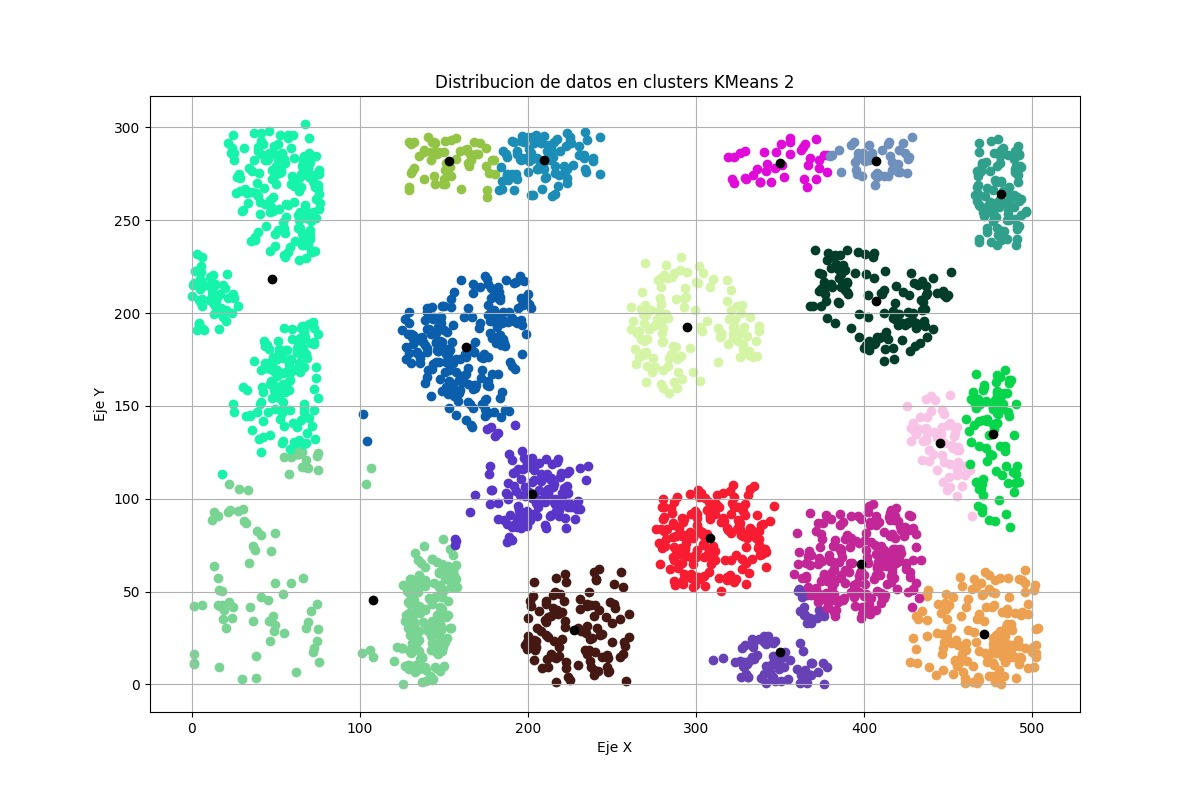
\includegraphics[width=1\linewidth]{figures/kmeans2.jpeg} % Adjust width as needed
    \caption{Distribucion de datos usando KMeans}
    \label{fig:kmeans2}
\end{figure}
\begin{figure}[htbp]
    \centering
    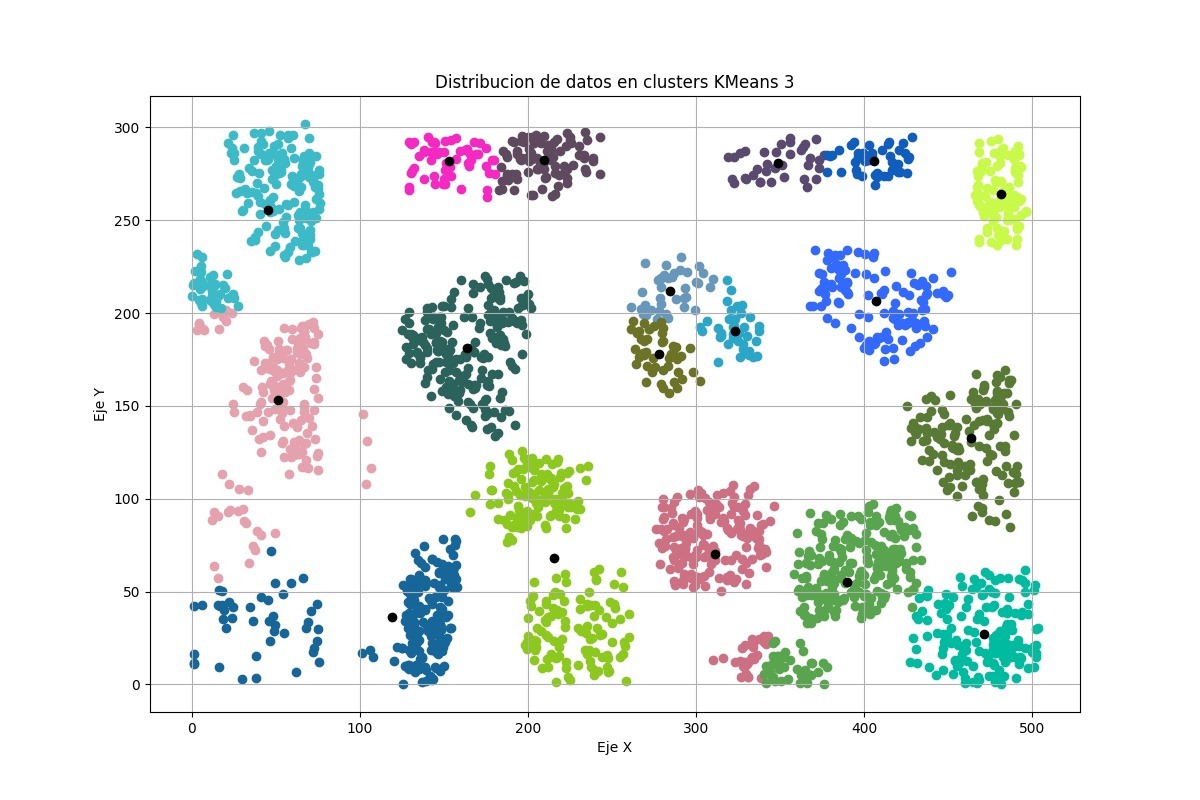
\includegraphics[width=1\linewidth]{figures/kmeans3.jpeg} % Adjust width as needed
    \caption{Distribucion de datos usando KMeans}
    \label{fig:kmeans3}
\end{figure}
\begin{figure}[htbp]
    \centering
    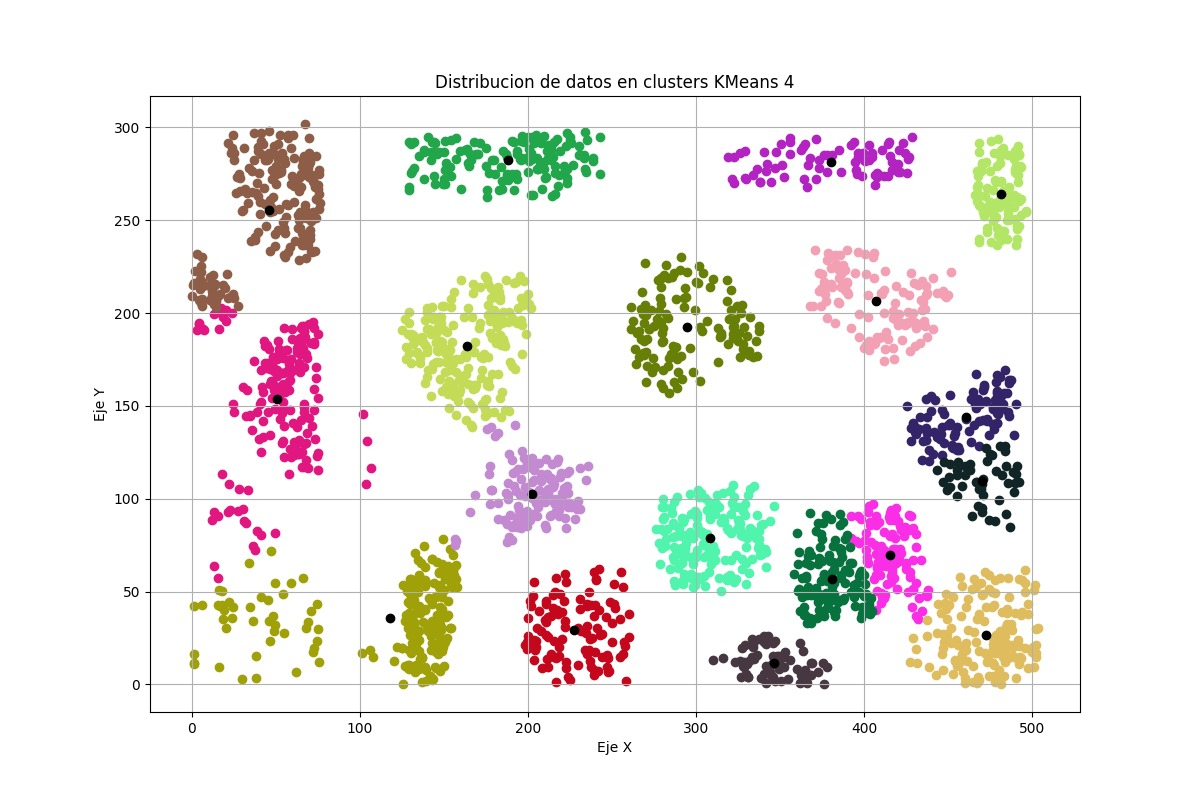
\includegraphics[width=1\linewidth]{figures/kmeans4.jpeg} % Adjust width as needed
    \caption{Distribucion de datos usando KMeans}
    \label{fig:kmeans4}
\end{figure}
\begin{figure}[htbp]
    \centering
    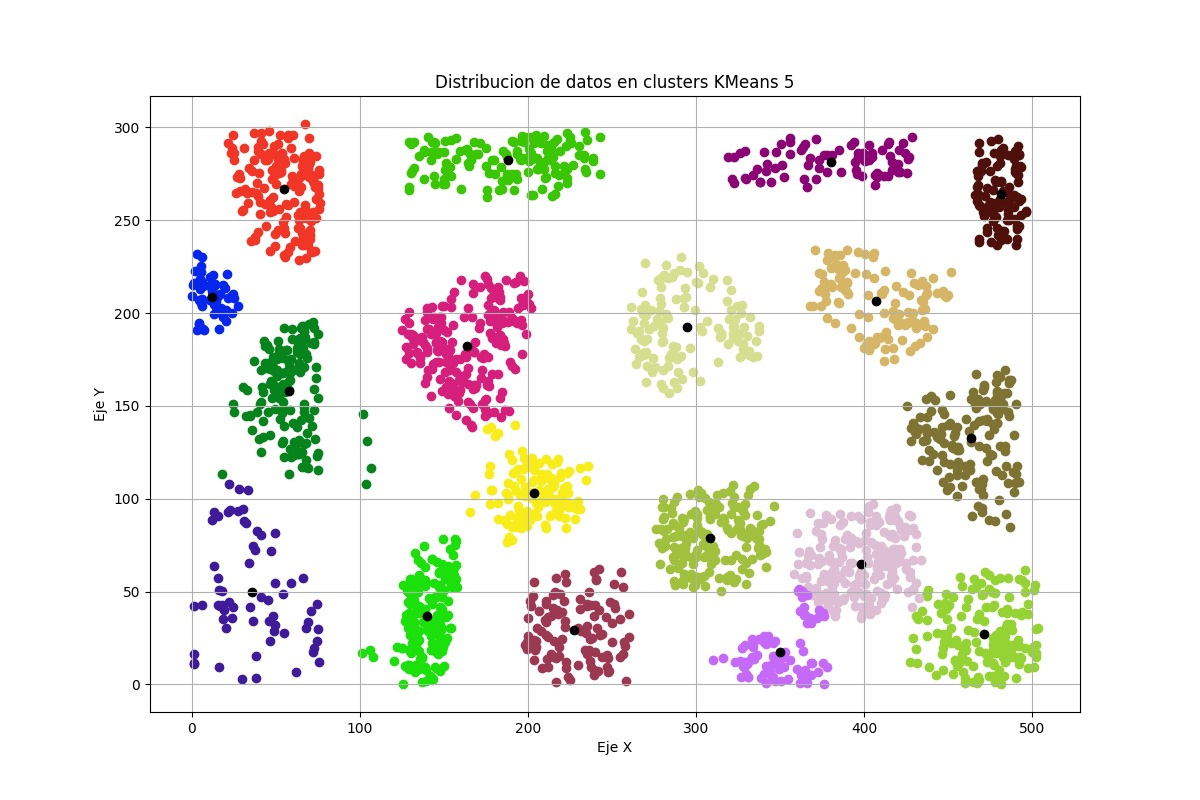
\includegraphics[width=1\linewidth]{figures/kmeans5.jpeg} % Adjust width as needed
    \caption{Distribucion de datos usando KMeans}
    \label{fig:kmeans5}
\end{figure}
\begin{figure}[htbp]
    \centering
    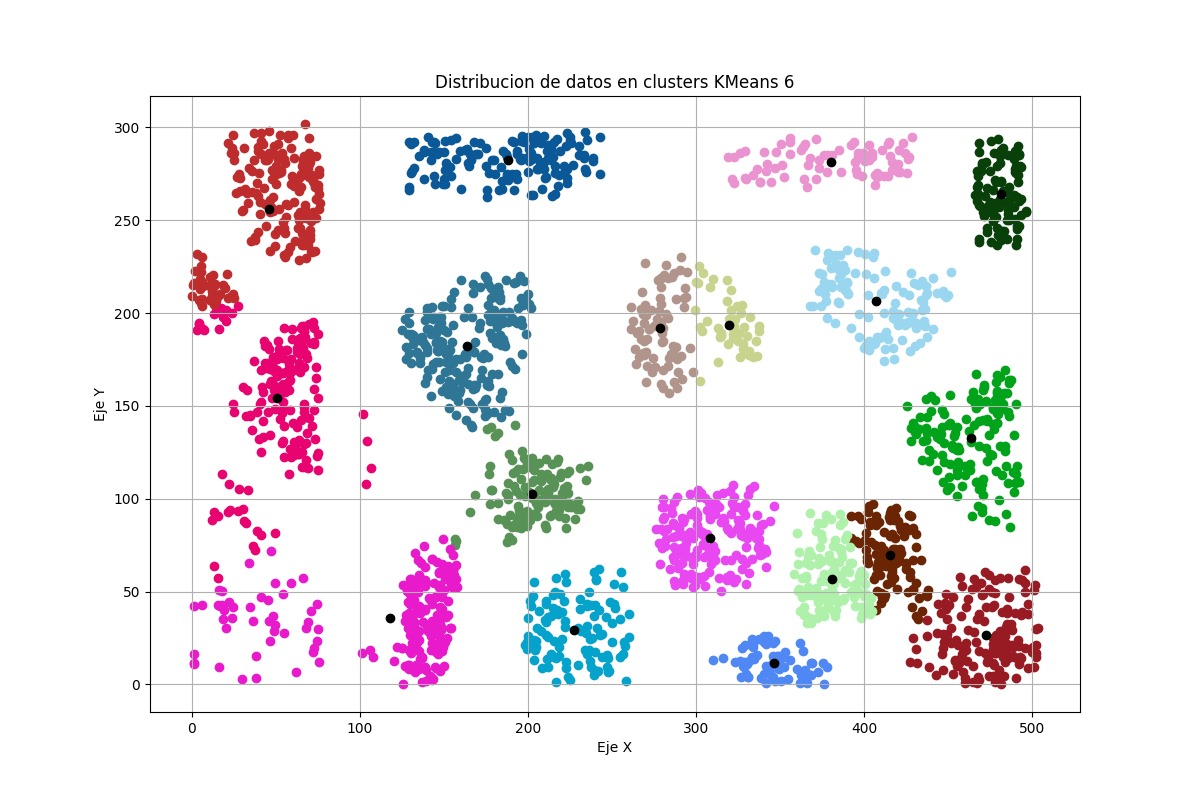
\includegraphics[width=1\linewidth]{figures/kmeans6.jpeg} % Adjust width as needed
    \caption{Distribucion de datos usando KMeans}
    \label{fig:kmeans6}
\end{figure}
\begin{figure}[htbp]
    \centering
    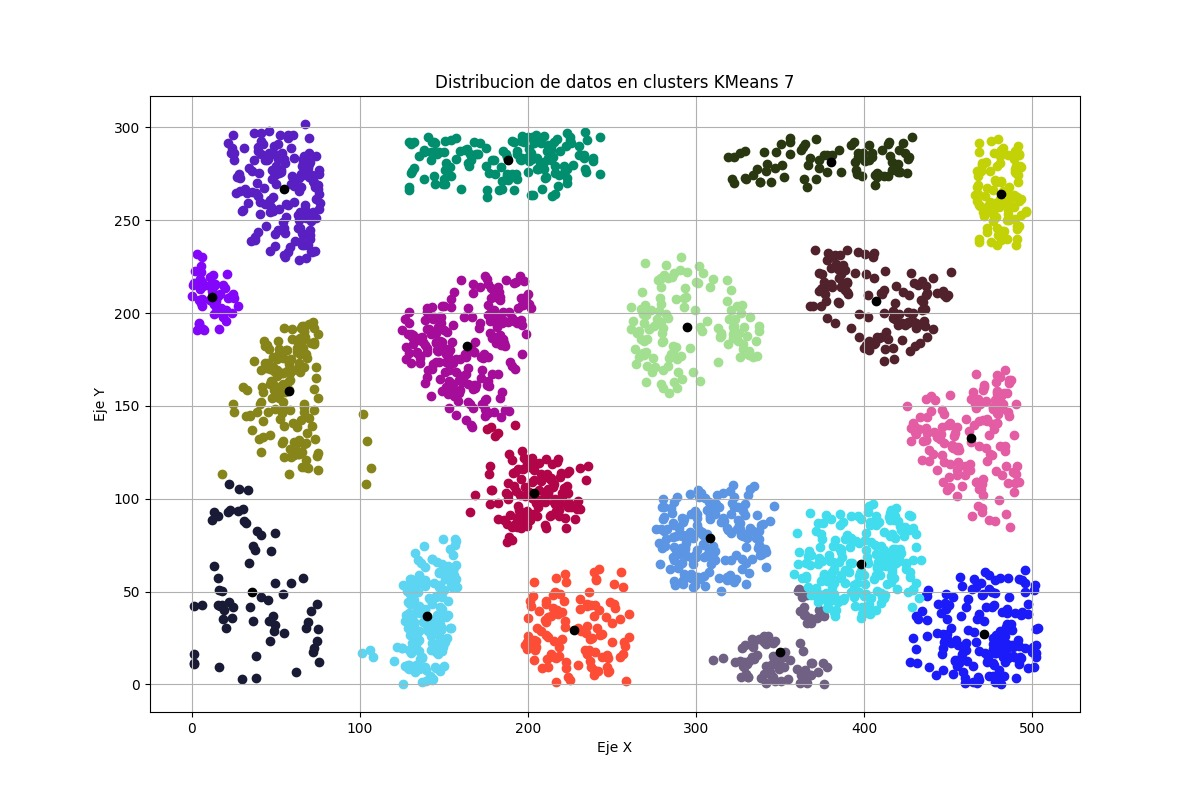
\includegraphics[width=1\linewidth]{figures/kmeans7.jpeg} % Adjust width as needed
    \caption{Distribucion de datos usando KMeans}
    \label{fig:kmeans7}
\end{figure}
\begin{figure}[htbp]
    \centering
    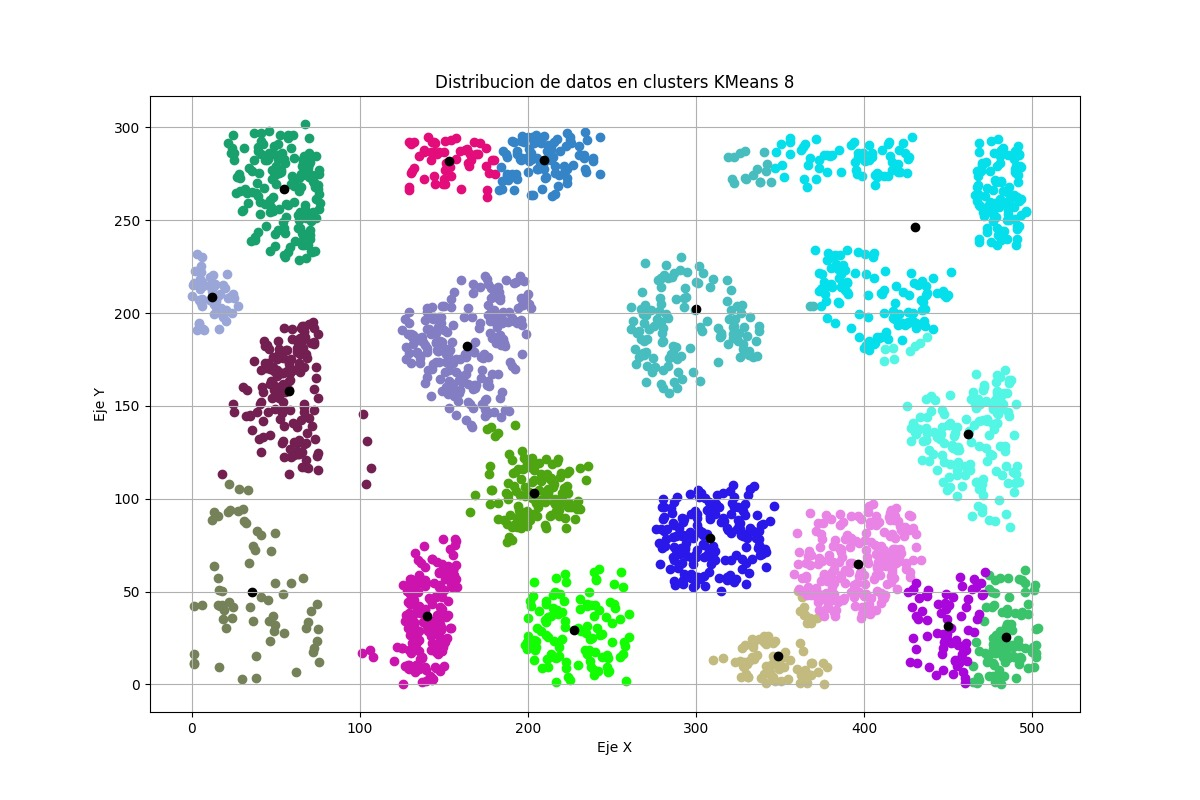
\includegraphics[width=1\linewidth]{figures/kmeans8.jpeg} % Adjust width as needed
    \caption{Distribucion de datos usando KMeans}
    \label{fig:kmeans8}
\end{figure}
\begin{figure}[htbp]
    \centering
    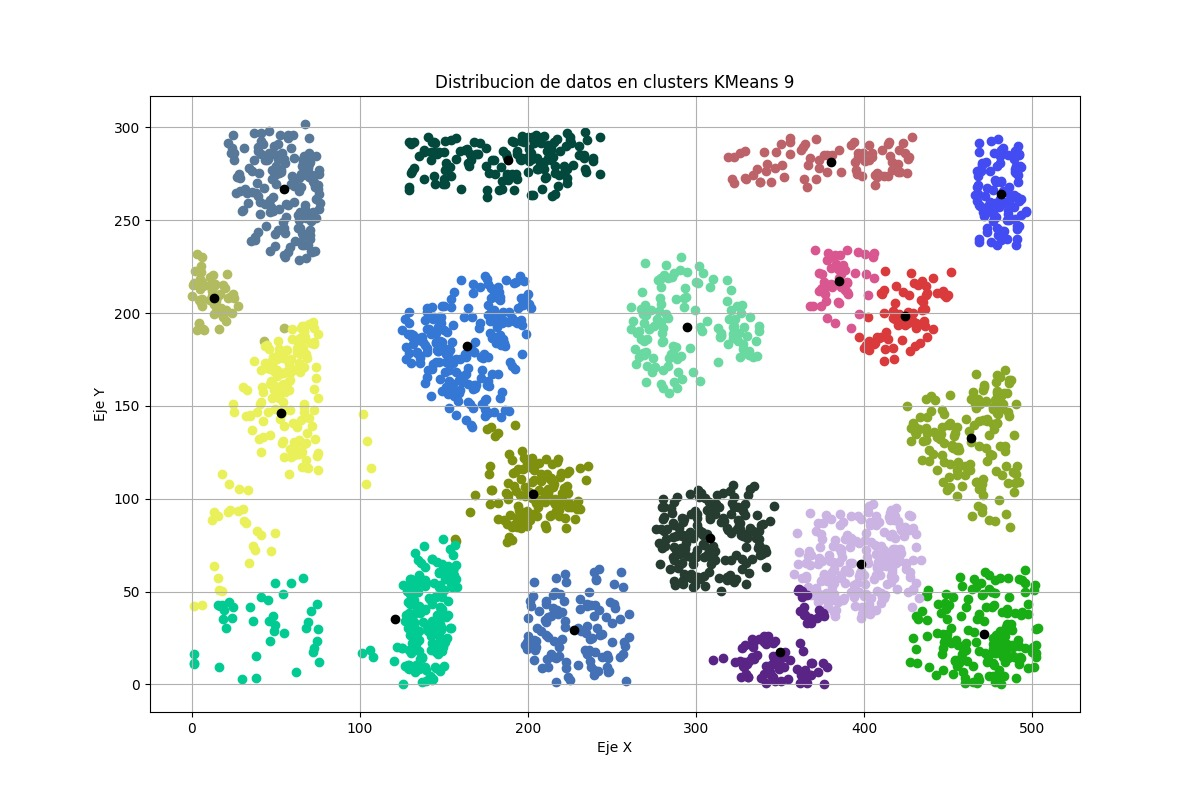
\includegraphics[width=1\linewidth]{figures/kmeans9.jpeg} % Adjust width as needed
    \caption{Distribucion de datos usando KMeans}
    \label{fig:kmeans9}
\end{figure}
\begin{figure}[htbp]
    \centering
    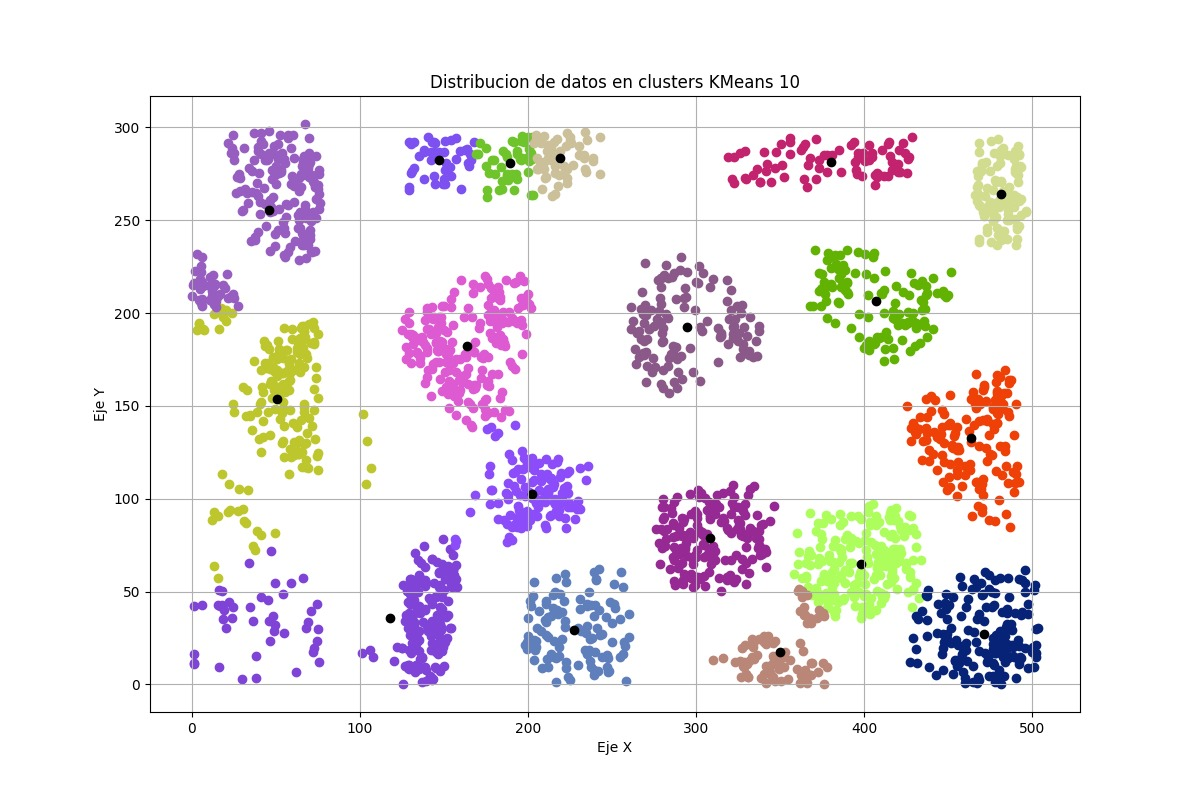
\includegraphics[width=1\linewidth]{figures/kmeans10.jpeg} % Adjust width as needed
    \caption{Distribucion de datos usando KMeans}
    \label{fig:kmeans10}
\end{figure}

\section{Consideraciones Adicionales}
\subsection{¿Por qué usar KDTrees y no otras estructuras?}
El uso de KDTree en el algoritmo KMeans se debe principalmente a su eficiencia en la búsqueda de vecinos más cercanos en espacios multidimensionales. Las siguientes razones destacan por qué KDTree es una opción preferida:
\begin{itemize}
    \item{Eficiencia en la Búsqueda.} KDTree ofrece una complejidad de búsqueda promedio de \(O(\log n)\) para encontrar el vecino más cercano, lo cual es significativamente más rápido que la búsqueda de fuerza bruta con \(O(n)\).
    \item{Estructura Adaptativa.} KDTree divide recursivamente el espacio de datos en regiones más pequeñas, lo que permite un acceso rápido y eficiente a los puntos de datos en consultas espaciales.
    \item{Construcción Relativamente Rápida.} La construcción de un KDTree tiene una complejidad de \(O(n \log n)\), lo que es manejable para conjuntos de datos de tamaño moderado.
\end{itemize}

\subsection{Otras Estructuras de Datos que Podrían Usarse}
Aunque KDTree es eficaz, hay otras estructuras de datos que también pueden ser utilizadas para mejorar la eficiencia del algoritmo KMeans:
\begin{itemize}
    \item{Ball Tree\cite{bhatia2010survey}.} Adecuada para datos en espacios de alta dimensionalidad, ya que agrupa puntos de datos en hiperesferas y ofrece consultas eficientes de vecinos cercanos.
    \item{Cover Tree\cite{beygelzimer2006cover}.} Especialmente útil para datos en espacios de muy alta dimensionalidad, ofreciendo consultas rápidas y una construcción eficiente.
    \item{VP Tree (Vantage Point Tree)\cite{fu2000dynamic}.} Optimizada para espacios métricos, adecuada para datos con una métrica de distancia específica, como la distancia Euclidiana.
    \item{R-Tree\cite{guttman1984r}\cite{bhatia2010survey}.} Comúnmente usada en sistemas de información geográfica (GIS) y bases de datos espaciales, es eficiente para consultas de rango y proximidad.
\end{itemize}

\subsection{¿Para Qué Tamaño de Datos en 2D es Beneficioso Usar un KDTree en el KMeans?}
El uso de KDTree es particularmente beneficioso para conjuntos de datos en 2D que son moderadamente grandes, típicamente en el rango de varios miles de puntos. Por ejemplo, para conjuntos de datos que varían entre 1000 a 2400 puntos, como se evaluó en este estudio, el KDTree proporciona una mejora significativa en la eficiencia de la búsqueda de vecinos más cercanos comparado con la búsqueda de fuerza bruta. Esto se debe a que en este rango de tamaño, el costo de construir y utilizar el KDTree es amortizado por la reducción en el número de comparaciones de distancia necesarias.

\subsection{¿Para Qué Valor de $k$ es Beneficioso Usar un KDTree en el KMeans?}
El uso de KDTree en KMeans es beneficioso para valores de $k$ moderados a grandes. En este estudio, se observó que la mejora en el tiempo de ejecución es notable para valores de $k$ desde 15 hasta 75 clusters. Para valores muy bajos de $k$ (como $k = 5$), la ventaja del KDTree no es tan significativa debido a que el número de comparaciones de distancia es ya relativamente bajo. En cambio, para valores más altos de $k$, el KDTree reduce de manera efectiva el tiempo necesario para asignar puntos a los centroides más cercanos, mejorando así la eficiencia general del algoritmo KMeans.

\section{Conclusiones}
En este estudio, se evaluó la eficiencia y efectividad de integrar la estructura de datos KDTree en el algoritmo KMeans. Las implementaciones de KMeans que utilizan KDTree muestran consistentemente tiempos de ejecución más bajos en comparación con las implementaciones de KMeans estándar para diversas combinaciones de tamaño de datos y cantidad de clústeres. Esto demuestra que el uso de KDTree para la búsqueda del vecino más cercano en el proceso de asignación de centroides en el algoritmo KMeans puede mejorar significativamente la eficiencia computacional, especialmente en conjuntos de datos más grandes o con una mayor cantidad de clústeres.

Al analizar los gráficos de desempeño, se observa que:
\begin{itemize}
    \item El incremento en el número de clusters tiene un impacto menor en el tiempo de ejecución cuando se utiliza KDTree en comparación con el KMeans estándar. Esto se debe a la optimización en la búsqueda de vecinos más cercanos que proporciona el KDTree.
    \item El aumento en la cantidad de datos afecta menos al desempeño del algoritmo cuando se emplea KDTree. La estructura KDTree permite una búsqueda más eficiente, manteniendo el tiempo de ejecución manejable incluso con grandes volúmenes de datos.
    \item La mejora en el tiempo de ejecución con KDTree es más evidente en espacios de baja a moderada dimensionalidad. En espacios de alta dimensionalidad, la eficiencia del KDTree disminuye, pero aún se observan beneficios en comparación con la implementación de fuerza bruta del KMeans.
\end{itemize}

Las mejoras en el tiempo de ejecución de KMeans con KDTree se pueden atribuir a la capacidad del KDTree para buscar estructuras de datos de árbol de manera eficiente, lo que reduce la complejidad computacional de asignar centroides a puntos de datos. Esta eficiencia es especialmente importante en conjuntos de datos distribuidos complejos o de alta dimensión.

No obstante, también se identificaron algunas limitaciones:
\begin{itemize}
    \item La necesidad de reconstruir el KDTree en cada iteración añade una sobrecarga computacional que debe ser considerada.
    \item En espacios de alta dimensionalidad, la eficiencia del KDTree disminuye, lo cual podría requerir el uso de técnicas adicionales de optimización.
\end{itemize}

En resumen, la integración de KDTree en el algoritmo KMeans ofrece una mejora sustancial en términos de eficiencia computacional, haciendo que el KMeans sea más viable para aplicaciones con grandes volúmenes de datos. Elegir utilizar KDTree en una implementación de KMeans puede proporcionar importantes beneficios de tiempo de ejecución, mejorando así la eficiencia de los algoritmos, especialmente en aplicaciones que necesitan procesar grandes cantidades de datos rápidamente. Sin embargo, la elección de utilizar KDTree debe ser considerada cuidadosamente en función de la dimensionalidad del espacio de datos y la estructura específica de los datos a analizar.



\bibliographystyle{IEEEtran}
\bibliography{bibliography/references}
\vspace{12pt}

\end{document}
